\documentclass[titlepage=firstiscover, captions=tableheading, bibliography=totoc]{scrartcl}
\usepackage[autostyle=true,german=quotes]{csquotes}
\usepackage{scrhack}
\usepackage{enumitem}
\usepackage{caption}
\usepackage[aux]{rerunfilecheck}
\usepackage{subcaption}
\usepackage{fontspec}
\usepackage[dvips]{graphicx}
\usepackage{floatflt,epsfig}

\usepackage{polyglossia}
\setmainlanguage{german}

\usepackage[unicode]{hyperref}
\usepackage{bookmark}
\title{Computational Physics}
\subtitle{Übungsblatt 7}
\author{
Miriam Simm\\
\texorpdfstring{\href{mailto:miriam.simm@tu-dortmund.de}{miriam.simm@tu-dortmund.de}\and}{,}
Katrin Bolsmann\\
\texorpdfstring{\href{mailto:katrin.bolsmann@tu-dortmund.de}{katrin.bolsmann@tu-dortmund.de}}{,}\\
\\
Mario Alex Hollberg\\
\texorpdfstring{\href{mailto:mario-alex.hollberg@tu-dortmund.de}{mario-alex.hollberg@tu-dortmund.de}}{}
}
\date{Abgabe: 15. Mai 2020}
\usepackage{amsmath}
\usepackage{amssymb}
\usepackage{mathtools}
\usepackage[
    math-style=ISO,
    bold-style=ISO,
    sans-style=italic,
    nabla=upright,
    partial=upright,
]{unicode-math}

\setmathfont{Latin Modern Math}

\usepackage[
  locale=DE,
  separate-uncertainty=true,
  per-mode=symbol-or-fraction,
]{siunitx}

\usepackage{multicol}
\setlength{\columnsep}{1pt} %space between columns

\usepackage{booktabs}
\usepackage[x11names, table]{xcolor}
\usepackage{graphicx}
\usepackage{grffile}
\usepackage{xfrac}
\usepackage{xcolor}

\usepackage{float}
\floatplacement{figure}{h}
\floatplacement{table}{h}
\usepackage[
  section,
  below,
]{placeins}

\usepackage{expl3}
\usepackage{xparse}
\ExplSyntaxOn
\NewDocumentCommand \E {} {\symup{e}}
\ExplSyntaxOff

% Literaturverzeichnis
\usepackage[
  backend=biber,
]{biblatex}
% Quellendatenbank
\addbibresource{literatur.bib}

\usepackage[
  version=4,
  math-greek=default,
  text-greek=default,
]{mhchem}


\raggedcolumns


\begin{document}

\maketitle

\section*{Aufgabe1: Lanczos-Algorithmus}

\subsection*{a)}
Der Lanczos-Algorithmus ist implementiert, sodass eine Tridiagonale Matrix $T$ berechnet wird. Mit einer $\textit{Eigen}$-Klasse werde dann Eigenwerte und Eigenvektoren berechnet. Leider kommen dabei keine sinnvollen Werte/Vektoren raus.

\subsection*{b)}
Die Hamilton-Matrix für eine Kette mit sechs Gitterplätzen sieht folglich aus:

\begin{pmatrix}
	0  & -t & 0			 & 0  & 0  & -t \\
	-t & 0  & -t	     & 0  & 0  &  0 \\
	0  & -t & \epsilon   & -t & 0  &  0 \\
	0  & 0  & -t		 & 0  & -t &  0 \\
	0  & 0  & 0			 & -t & 0  &  -t \\
	-t & 0  & 0			 & 0  & -t &  0 
\end{pmatrix}

\subsection*{c)}
Für sehr große $N$ könnte man eine Sparse-Matrix (dünnbesetzte Matrix) benutzen.

\section*{Aufgabe2: Federkette}
Gegeben sei eine freie lineare Federkette mit Punktmassen $m_i$, Federkonstanten $k_j$ und Federruhelängen $l_j$ mit $i \in \{1, ..., N\}$ und $j \in \{1, ..., N-1\}$.
\begin{figure}[h]
    \centering
    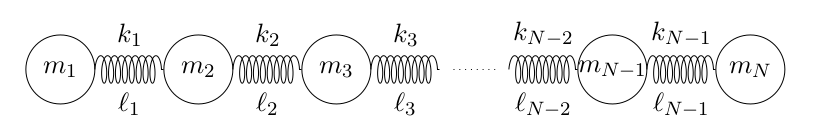
\includegraphics[width=0.8\textwidth]{Federkette.png}
    \label{fig:1a}
\end{figure}

\noindent
Allgemein gilt

\begin{align*}
  m_1\ddot{x}_1 &= k_1(x_2 - x_1) \\
  m_i\ddot{x}_i &= -k_{i-1} (x_i - x_{i-1}) + k_i(x_{i+1}-x_i) \\
  m_N\ddot{x}_N &= -k_{N-1}(x_N - x_{N-1}) \\
\end{align*}

\noindent
Damit ergibt sich das Differentialgleichungssystem

\begin{equation*}
  \left(\begin{array}{c} \ddot{x}_1 \\ \ddot{x}_2 \\ \vdots \\ \ddot{x}_N \end{array}\right)\, = \,
  \underbrace{\left(
        \begin{array}{ccccc}
          \frac{-k_1}{m_1} & \frac{k_1}{m_1} & 0 & \cdots & \\
          \frac{k_1}{m_2} & \frac{-k_2-k_1}{m_2} & \frac{k_2}{m_2} & 0 & \cdots \\
          & & \ddots & & \\
          & & & \frac{k_{N-1}}{m_N} & \frac{-k_{N-1}}{m_N}\\
        \end{array}\right)}_{\underline{\underline{A}}}
        \left(\begin{array}{c} x_1 \\ x_2 \\ \vdots \\ x_N \end{array}\right)
\end{equation*}

Zum Lösen des Differentialgleichungssystems wählen wir den Ansatz $x_i(t) \sim e^{i\omega t}$, womit für die Ableitung direkt $\ddot{\vec{x}} = -\omega^2 \vec{x}$ folgt. Durch Einsetzen von $\ddot{\vec{x}}$ ergibt sich aus dem Differentialgleichungssystem eine Eigenwertgleichung.

\begin{equation*}
  \underline{\underline{A}}\vec{x} = -\omega^2\vec{x}
\end{equation*}

\noindent
Die Eigenfrequenzen entsprechen also der Wurzel der negativen Eigenwerte. Das Eigenwertproblem wurde in Aufgabe2.cpp für
\begin{align*}
  m_i &= i \\
  k_j &= N-j \\
  l_i &= |5-j|+1
\end{align*}

\noindent
gelöst und für die Eigenfrequenzen die Werte

\FloatBarrier
\begin{table}[h]
    \centering
    \begin{tabular}{l}
        \textbf{$\qquad \omega$} \\
        \toprule 3.95439 \\ 2.62228 \\ 1.95382 \\ 1.51083 \\ 1.17586 \\ 0.901365 \\ 0.663369 \\ $1.4585\cdot 10^{-9}$ \\ 0.44762 \\ 0.243446 \\
        \bottomrule
    \end{tabular}
\end{table}
\noindent
\FloatBarrier
\noindent
berechnet. Aufgefallen ist uns, dass die Federruhelängen nicht zur Berechnung der Eigenfrequenzen benötigt wurden. Diese sind also unabhängig von den Anfangsbedingungen. $\vec{l}$ wird lediglich benötigt, um die explizite Lösung des Differentialgleichungssystems $\vec{x}$ aufzustellen, diese müssen dann $\vec{x}(0) = \vec{l}$ erfüllen.

\section*{Aufgabe3: Integrationsroutinen und eindimensionale Integrale}

\end{document}
